\subsubsection{Dijkstra}

L'algorisme Dijkstra's és un algorisme que ens serveix per trobar el camí més curt des del node inicial fins a tots els nodes del graf. \newline

Suposant que les arestes tenen llargades, quan ens referim al camí més curt no ens referim al camí on hem de travessar menys arestes sinó al camí el qual la llargada total de les arestes per les quals passem és la més curta. \newline

Per entendre-ho millor, imaginem que volem anar a París, Anglaterra i Roma des de Barcelona (les ciutats representen nodes i les carreteres arestes), per fer-ho hem de passar per moltes ciutats intermediàries i hi ha moltes maneres diferents d'arribar-hi, però nosaltres volem agafar el camí en el qual la distància total entre ciutats intermediàries sigui mínima per tal de recórrer el menor nombre de quilòmetres, esbrinar-ho seria una feina molt tediosa, ja que hi ha masses carreteres i combinacions possibles, per sort tenim el Google Maps que amb l'ús de l'algorisme Dijkstra's ja ho resol. \newline

Posarem com a exemple el funcionament de l'algorisme Dijkstra amb el següent graf (figura 16).

(En vermell les distàncies fins a cada node, en negre el nombre del node i distància de cada aresta)
\newline

\begin{center}
    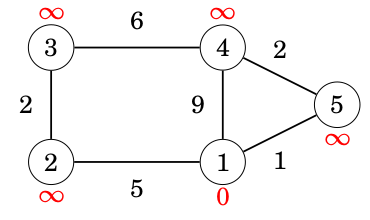
\includegraphics[width=.5 \textwidth]{grafDij1.png}
    
    \caption{\emph{Figura 16: Graf amb llargades. Font: \url{https://cses.fi/book/book.pdf}}}
\end{center}

Primerament, guardem distància infinita a tots els nodes menys al node inicial, que li posem distància 0.

A cada pas, l'algorisme escull un node que no ha estat processat encara i que la seva distància és la menor possible. En aquest cas seleccionem el node 1.

Cada vegada que un node és seleccionat, l'algorisme travessa totes les arestes que comencen al node i escurça les distàncies cap a altres nodes mitjançant aquestes:

\begin{center}
    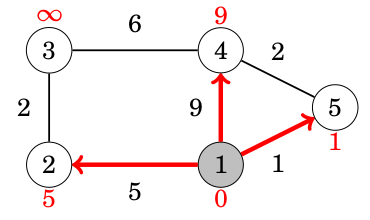
\includegraphics[width=.5 \textwidth]{grafDij2.png}
    
    \caption{\emph{Figura 17: Graf amb llargades. Font: \url{https://cses.fi/book/book.pdf}}}
\end{center}

En aquest cas, les arestes del node 1 han reduït les distàncies fins als nodes 2,4 i 5 que ara passen a ser 5,9 i 1.

Seguidament, processem el node 5, que ens redueix la distància fins al node 4 de 9 fins a 3, ja que és més òptim fer un camí de distància 2+1 = 3 que de distància 9.

\begin{center}
    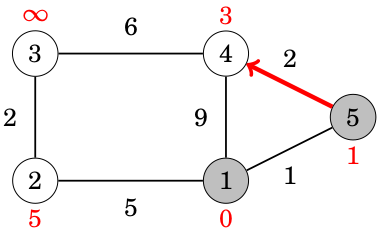
\includegraphics[width=.5 \textwidth]{grafDij3.png}
    
    \caption{\emph{Figura 18: Graf amb llargades. Font: \url{https://cses.fi/book/book.pdf}}}
\end{center}

Ara toca processar el node 4 que ens redueix la distància fins al node 3.

\begin{center}
    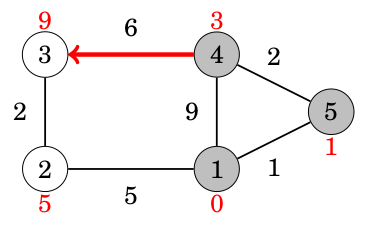
\includegraphics[width=.5 \textwidth]{grafDij4.png}
    
    \caption{\emph{Figura 19: Graf amb llargades. Font: \url{https://cses.fi/book/book.pdf}}}
\end{center}

Aquest procés el repetim dues vegades més amb els nodes 2 i 3, finalment obtindríem les distàncies òptimes cap a tots els nodes i el graf quedaria de la següent manera.

\begin{center}
    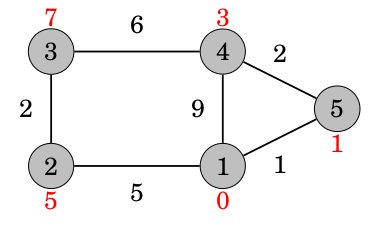
\includegraphics[width=.5 \textwidth]{grafDij5.png}
    
    \caption{\emph{Figura 20: Graf amb llargades. Font: \url{https://cses.fi/book/book.pdf}}}
\end{center}

La següent implementació de l'algorisme de Dijkstra calcula les distàncies mínimes des d'un node $x$ als altres nodes del graf.

Una implementació eficient de l'algorisme de Dijkstra requereix trobar de manera eficient el node de distància mínima que no s'ha processat encara. L'estructura de dades adequada és una cua de prioritats que conté els nodes ordenats per distància. Amb una cua de prioritats trobem el següent node a processar en temps $O(\log n)$.

El graf s'emmagatzema com a llistes d'adjacència de manera que $adj[a]$ conte un parell $(b, w)$ quan hi ha una aresta del node $a$ fins al node $b$ amb pes $w$.

El vector $dist$ conte la distància a cada node.

Inicialment, la distància és 0 al node inicial i $\infty$ a tots els altres nodes.

\begin{lstlisting}
vector<vector<pair<int,int>>> adj; // llista d'adjacència
vector dist; // llista de distàncies
int INF = 10e9;

for (int i=1; i<n; i++)
    dist[i] = INF; // marquem distància infinita a
                   // tots els nodes menys el 0

priority_queue<pair<int,int>> cua; // distància - node
cua.push({0, 0}); // afegim a la cua node 0 amb distància 0

// comencem el Dijkstra's

while (!cua.empty()){
    int nodeActual = cua.top().second; 
    // agafem el node amb menys distància
    int distanciaActual = cua.top().first
    cua.pop(); // traiem el node de la cua
    
    if (abs(distanciaActual) > dist[nodeActual]) continue;
    // si el valor absolut de la distància del nodeActual és menor,
    // no la volem actualitzar
    
    for (auto u : adj[nodeActual]){ // mirem els nodes adjacents
        int nodeAdjacent = u.first;
        int distancia = u.second;
        
        if (dist[nodeActual] + distancia < dist[nodeAdjacent]){
            // si podem acurtar la distancia al nodeAdjacent mitjançant
            // el nodeActual, l'actualitzem
            dist[nodeAdjacent] = dist[nodeActual] + distància;
            // afegim la nova distància i el nodeAdjacent
            cua.push({-dist[nodeAdjacent], nodeAdjacent});
        }
    }
}

\end{lstlisting}

Cal recalcar que la complexitat temporal de la implementació anterior és $O(n + m \log m)$, per
què l'algorisme passa per tots els nodes del graf i afegeix, per cada aresta, com a màxim una distància a la cua de prioritats.